\section{Motion Planning Module(Catherine)}

%Motivation (why did you do it, who should care about it)
%Clearly state your contributions
%Technical details of what you did, with a focus on what's novel.
%Experimental results (if you did any experiments)
%Discussion (what is interesting about the results)

%This component is divided into two subsections:
%\begin{enumerate}%[label=\thesection.\arabic*]
%\item Trajectory Planner for robot arm trajectory planning, and
%\item Trajectory Executor for robot arm trajectory execution.
%\end{enumerate}

The motion planning module can be separated into three submodules as shown in Fig.~\ref{fig:plan}.

\begin{figure}[ht!]%[H]
\centering
{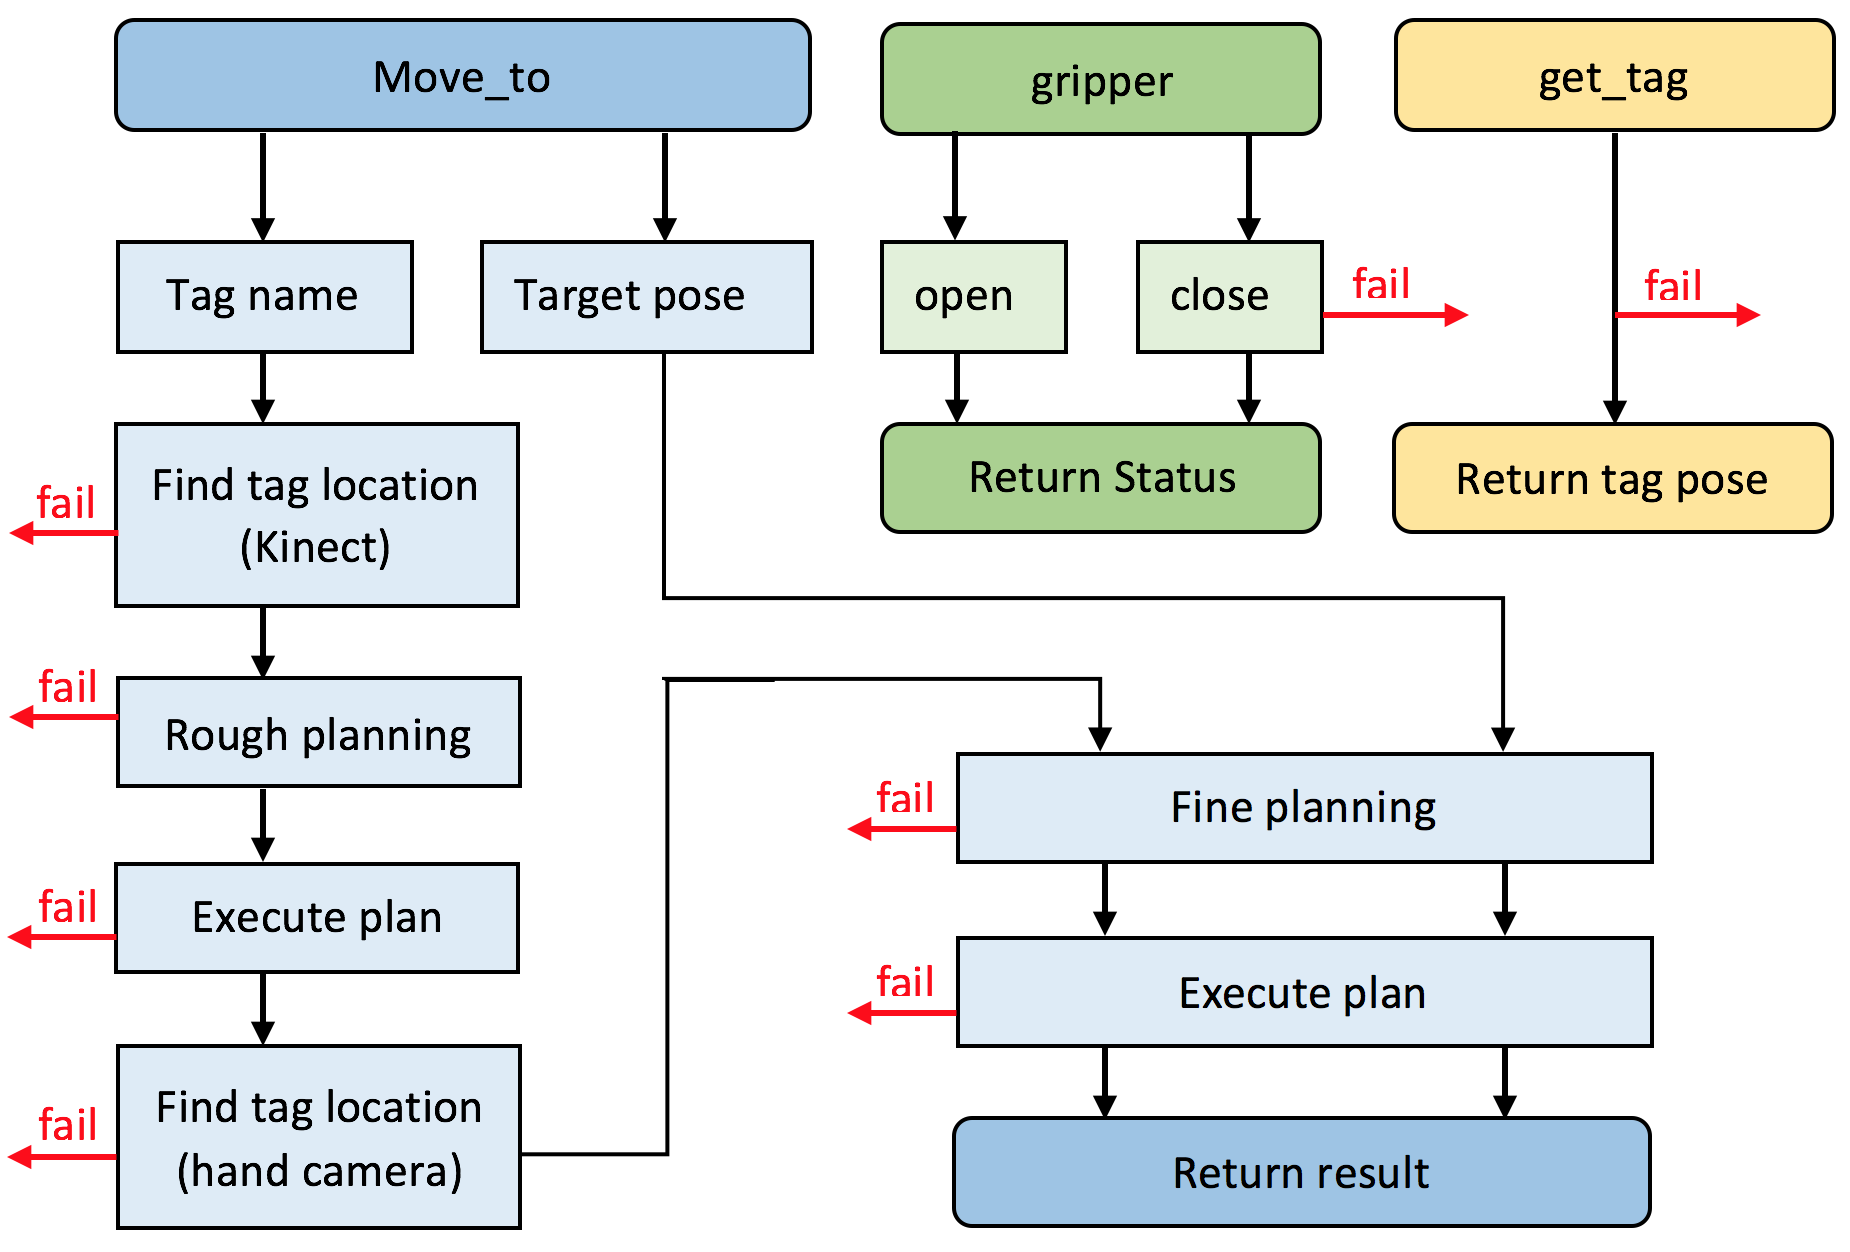
\includegraphics[width=0.95\columnwidth]{pics/motion_planning_flow.png}}
\caption{Motion Planning Module}
\label{fig:plan}
\end{figure}


\subsection{Trajectory Planner (move\_to module)}

During execution, the task planner requests the path planner to create trajectory plans for one or more robot arms. The planner aims to find a plan that (i) each arm starts at its initial configuration, and (ii) each arm ends with each robot end effector within a certain distance from the final desired workspace position. 

There are a variety of path planning algorithms developed in the community~\cite{DBLP:books/daglib/0016830} and some algorithms are adapted for finding robot arm trajectories. 
Researchers have proposed sampling-based approaches with probabilistic completeness such as the Rapidly-Exploring Random Tree (RRT) algorithm~\cite{VahrenkampBAKD09} to find trajectories for robot arms. Others have used Probabilistic RoadMaps (PRM) that work with high-dimensional spaces~\cite{KavrakiSLO96} but the algorithm requires pre-computation of the roadmap and no dynamic obstacles in the environment. In this work, we do not conduct pre-processing and the other arms can temporarily be obstacles in the environment so we are using an improved version of RRT, RRT-Connect~\cite{KuffnerL00} to find trajectories for the robot arms.


Our work leverages the existing open-source planning software for manipulation, MoveIt! \cite{moveit} with the Open Motion Planning Library (OMPL)~\cite{sucan2012the-open-motion-planning-library} to plan trajectories for the robot arms. 


\subsubsection{Objects to Avoid in Trajectory Planning}~\\
The major objects to avoid in path planning are the table and all the modules excluding the target module, as shown in Fig.~\ref{fig:realBaxter}. In this project, we have explored two different ways to model objects in the world. 

\paragraph{Octamap}\label{obstacle-octamap}
For our first attempt, we subscribe to the depth information of a Kinect facing the robot and create an octamap around the robot. An octamap is a 3-D occupany grid that builds an obstacle map around the source, in this case the Kinect, and updates over time with new information of the evolving environment. Figure~\ref{fig:octamap} shows an example of the octamap around Baxter.

Since the modules are modeled as obstacles in the octamap, to approach and grasp the module, we remove the target module from the octamap through inserting a module-like scene object into the workspace (Fig ????????). The octamap automatically subtracts any scene objects and by excluding the module object from the collision checking in trajectory planning, MoveIt! can find a path to the module.

\paragraph{Table object}\label{obstacle-table}
Since the environment of the workspace is given, the other way to model obstacles in the environment is simply adding a table object right in front of Baxter. 

We compared the performance of the two approaches for modeling obstacles. It turns out clustering of modules could be a problem when using an octamap and no plans can be found. If we simply model the environment with only a table in front, the resulting plan may sometimes touch the other modules. However, looking at Fig.~\ref{fig:table}, notice that the table object is a pretty good representation of the obstacle information from the octamap. Since the modules are movable in the workspace, we determined that it will be better to get a plan most of time and we go on with ~\ref{obstacle-table} to model obstacles. 

%\quad
%\quad
\begin{figure}[ht!]%[H]
\centering
\subfloat[Real Scenario of Baxter with modules on a table]{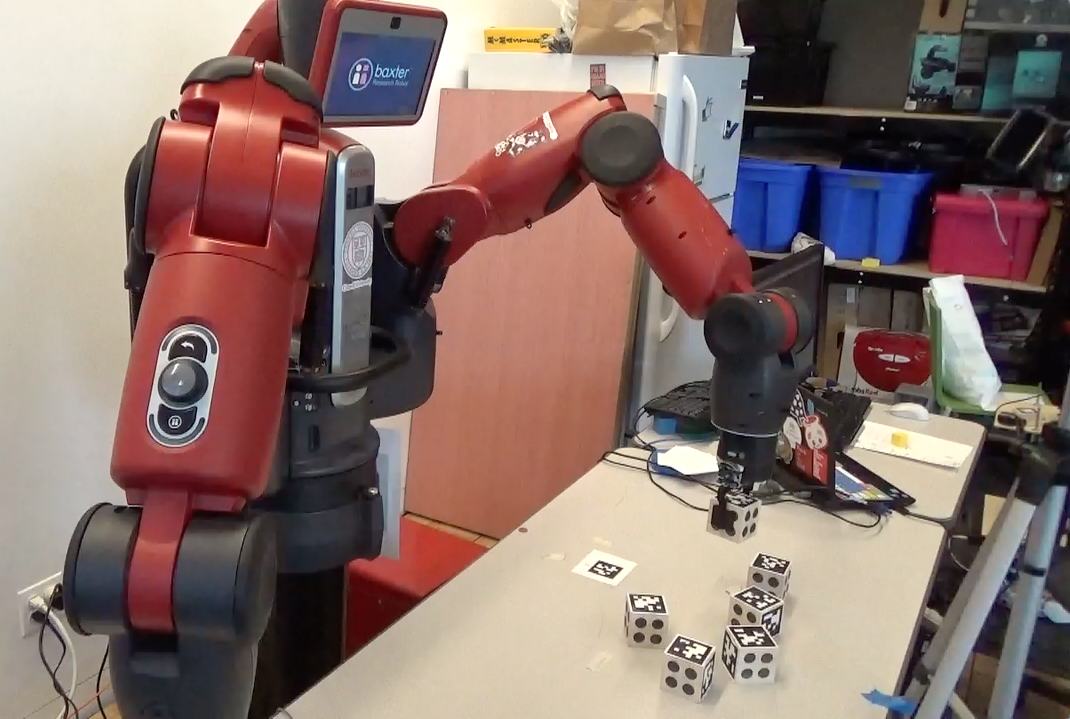
\includegraphics[width=0.31\columnwidth]{pics/baxter_real_table.png}\label{fig:realBaxter}}\hspace{0.1cm}
\subfloat[Octamap from depth data of Kinect in Rviz]{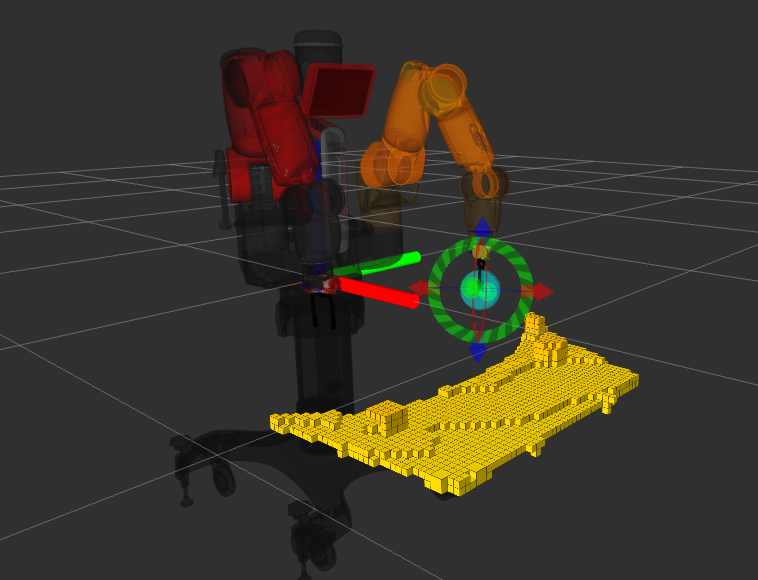
\includegraphics[width=0.31\columnwidth]{pics/baxter_with_octamap.png}\label{fig:octamap}}\hspace{0.1cm}
\subfloat[Octamap from depth data of Kinect with a table object inserted in Rviz]{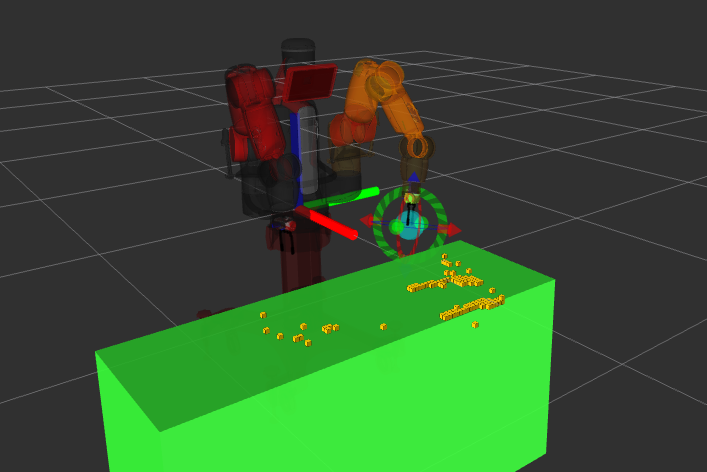
\includegraphics[width=0.31\columnwidth]{pics/baxter_with_table.png}\label{fig:table}}
\\
\caption{Modeling obstacles in trajectory planning}
\end{figure}



\subsubsection {transformation}~\\
First, we obtain a rough location of the module from the Kinect sensor based on camera feed. Then, we transform the tag pose such that the final location of the gripper will be approximately above the module,  and also flip the axis of the module and this will be the goal pose of the gripper in consideration. The transformation can be formulate with the following two questions.

$\mathrm{endEffectorPose}=
\begin{bmatrix}
    X_{offset} \\
    Y_{offset} \\
    Z_{offset}
\end{bmatrix}
+
\begin{bmatrix}
    \mathrm{tagPose}_{x} \\
    \mathrm{tagPose}_{y} \\
    \mathrm{tagPose}_{z} \\
\end{bmatrix}
$

$q_{tag/world} = (r_t,\overrightarrow{v}_t)$
$q_{goal/world} = (r_g,\overrightarrow{v}_g)$
$q_{goal/world} = (r_g,\overrightarrow{v}_g)$

$(|o|,\overrightarrow{orientation}_{tag/world}) = $

$\mathrm{orientation}=
\begin{bmatrix}
    1 & 0 & 0 & X_{offset} \\
    0 & 1 & 0 & Y_{offset} \\
    0 & 1 & 0 & Z_{offset} \\
    0 & 0 & 0 & 1 \\
\end{bmatrix}
\begin{bmatrix}
    1 & 0 & 0 & X_{pose} \\
    0 & 1 & 0 & Y_{pose} \\
    0 & 1 & 0 & Z_{pose} \\
    0 & 0 & 0 & 1 \\
\end{bmatrix}
$

%figure for difference between kinect pose and pose from camera

\subsubsection {two-step planning}~\\
Through testing our approach, our group have noticed that the camera information from a Kinect sensor does not give an accurate position of the modules with the recognition of AprilTags~\cite{Olson11}. The position of the module from Kinect is off by about 5cm and this is not good enough for the arm and gripper to arrive at the module location and grasp the module.
 
 %%%%%%%%%
In this work, we propose a two-step trajectory planning. 

Once the robot arms moves to the 'rough' location, now the robot can use the camera on its hand to obtain a better location estimate of the module.  With a more accurate location, the system then do a fine planning to the grasp location of the module. 

If the planner finds a plan, it returns the joint-space trajectory for each arm. If the planning exceeds the time limit, then the planner aborts and returns no trajectories. 

\subsection{Failures}
Since RRT is probabilistic complete, it may not find a path given a finite time horizon. As a result, it is useful to provide feedback to the client that the planning failed. In our case, we can find out if a plan is found and return the status of each planning to the client so client can execute other things when waiting for the execution of the plan. 


The pose of each module comes from either an external Kinect or from the two cameras on the robot hand. Since poses detection are inaccurate if too far from the module. Thus, we came up with a two-step planning.


The two steps both leverage RRT to conduct the planning. First the algorithm does a rough planning to a certain distance above the module given a location from the Kinect. If the planning is successful, then our system retrieves the tag pose again but this time using the camera on the hand. Since the arm is roughly on the top of the module, this results in a better approach towards the module and at the end grasp the module

% To insert: show difference in kinect pose and pose from hand. 




Our motion will always come from the top in this system. 


The action server lib is can respond to five different action requests
\begin{itemize}
\item open gripper
\item close gripper
\item go to a pose that the hand camera can see the tag, with a fix pose pre-given
\item go to a tag
\item get tag pose
\end{itemize}

the section also in charge of getting the pose of different modules if receiving a request from the high-level planner or the joint controller

other attempts
\begin{itemize}
\item also tried broadcasting the goal location of the robot to tf and then fetch it, but then there is a lot of overhead and it will be easier doing transformation leveraging the tf.transformation module.
\item also played with the inverse kinematic library (pyKDL) before but when switch it moveit, all the inverse kinematics are handled by Moveit.
\item originally tried to generate waypoints of trajactory. To populate points on the RRT tree, but collision detection is using FCL but moveit set up the environment/scene so using moveit now.
\item create object and then removing to from collision matrix. in this case, the robot can contact the object and the octamap is cleared at the point. The downside was the filtering wasn't good around the grippers. Also adding a table gives a close approximation. 
\end{itemize}

\subsection{open and close gripper}

%--------- old %%%%


First, we plan to try two different RRT approaches and compare their performance. With RRT, there are still multiple ways to generate a trajectory plan.
One of them is to generate trajectory plan synchronously.
For example, if there are four arms available for a task, or two Baxters, then the planning could be synchronous, i.e, we plan all the arms at the same time and each node in RRT stores the joint information of the four arms. With each arm having 7 degrees of freedom (DoF), a synchronous planning has up to 28 degrees of freedom.
With this approach, assuming the workspace has no other obstacles, collision avoidance with the other arms is taken care of during the planning phase so it is unnecessary during trajectory execution.  
The trade off of synchronous planning is that one arm may wait for the others even though its trajectory is found.

Alternatively, another way would be to first create a plan each arm separately and assign priorities to each arm. An arm then replans only when its trajectory intersects with the plan of another arm with a higher priority. Compared with the synchronous approach, each planning contains 7 degrees of freedom but re-plannings of trajectory can go up to (n-1) times, with n being the number of arms. 

Second, we plan to create our own version of RRT planner and also utilize off-the-shelf library with RRT such as the Open Motion Planning library (OMPL)~\cite{sucan2012the-open-motion-planning-library} to find out the one with better performance.
Compared with creating our own RRT planner, OMPL has lots of planning algorithms available, but most examples of OMPL work with single robot or arm and planning for multiple arms simultaneously with OMPL may be unfeasible. We plan to learn more about OMPL and then decide if we are creating our own RRT planner or we are using OMPL to build our planner.

Finally, RRT is only a template for planning and we need to complete the template with ways to propagate a trajectory and smoothen the resulting trajectory. 
During the planning phrase, we plan to optimize the final trajectory by reducing the difference in joint angles between two nodes in the RRT tree. We use inverse kinematics find robot joint angles given a desired location of the end effector.


%To conduct a path planning of the robot arms, the planner takes in:

%\begin{itemize}
%\item the number of arms we are planning, 
%\item the starting joint configurations of each arm, and
%\item the final workspace positions of robot end effectors.
%\end{itemize}



\subsection{Trajectory Executor}

Besides a trajectory planner, the person in charge of this component also creates a trajectory executor that executes any given trajectory.
Once the task planner receives a plan, it can invoke the trajectory executor to execute the path. The executor takes in a joint-space trajectory and notifies the task planner when it finishes the execution. The task planner then invokes planning by the action planner in the next section to conduct fine and accurate objects manipulation.
